\documentclass[10pt,letterpaper]{article}

\providecommand{\main}{.}
\usepackage{pslatex}
\usepackage{graphicx}
\usepackage{multicol}
\usepackage{blindtext}
\usepackage{tablefootnote}
\usepackage{hyperref}
\usepackage{tipa}
\usepackage{cogsci}
\usepackage{booktabs}
\usepackage[table,usenames,dvipsnames]{xcolor}
\usepackage[style=apa]{biblatex}
\DeclareNameAlias{sortname}{family-given}
\addbibresource{qp1.bib}
\usepackage{gb4e}

\graphicspath{{\main/figures/}{figures}}

\begin{document}
	
 	\begin{figure}[h]
 	\centering
 	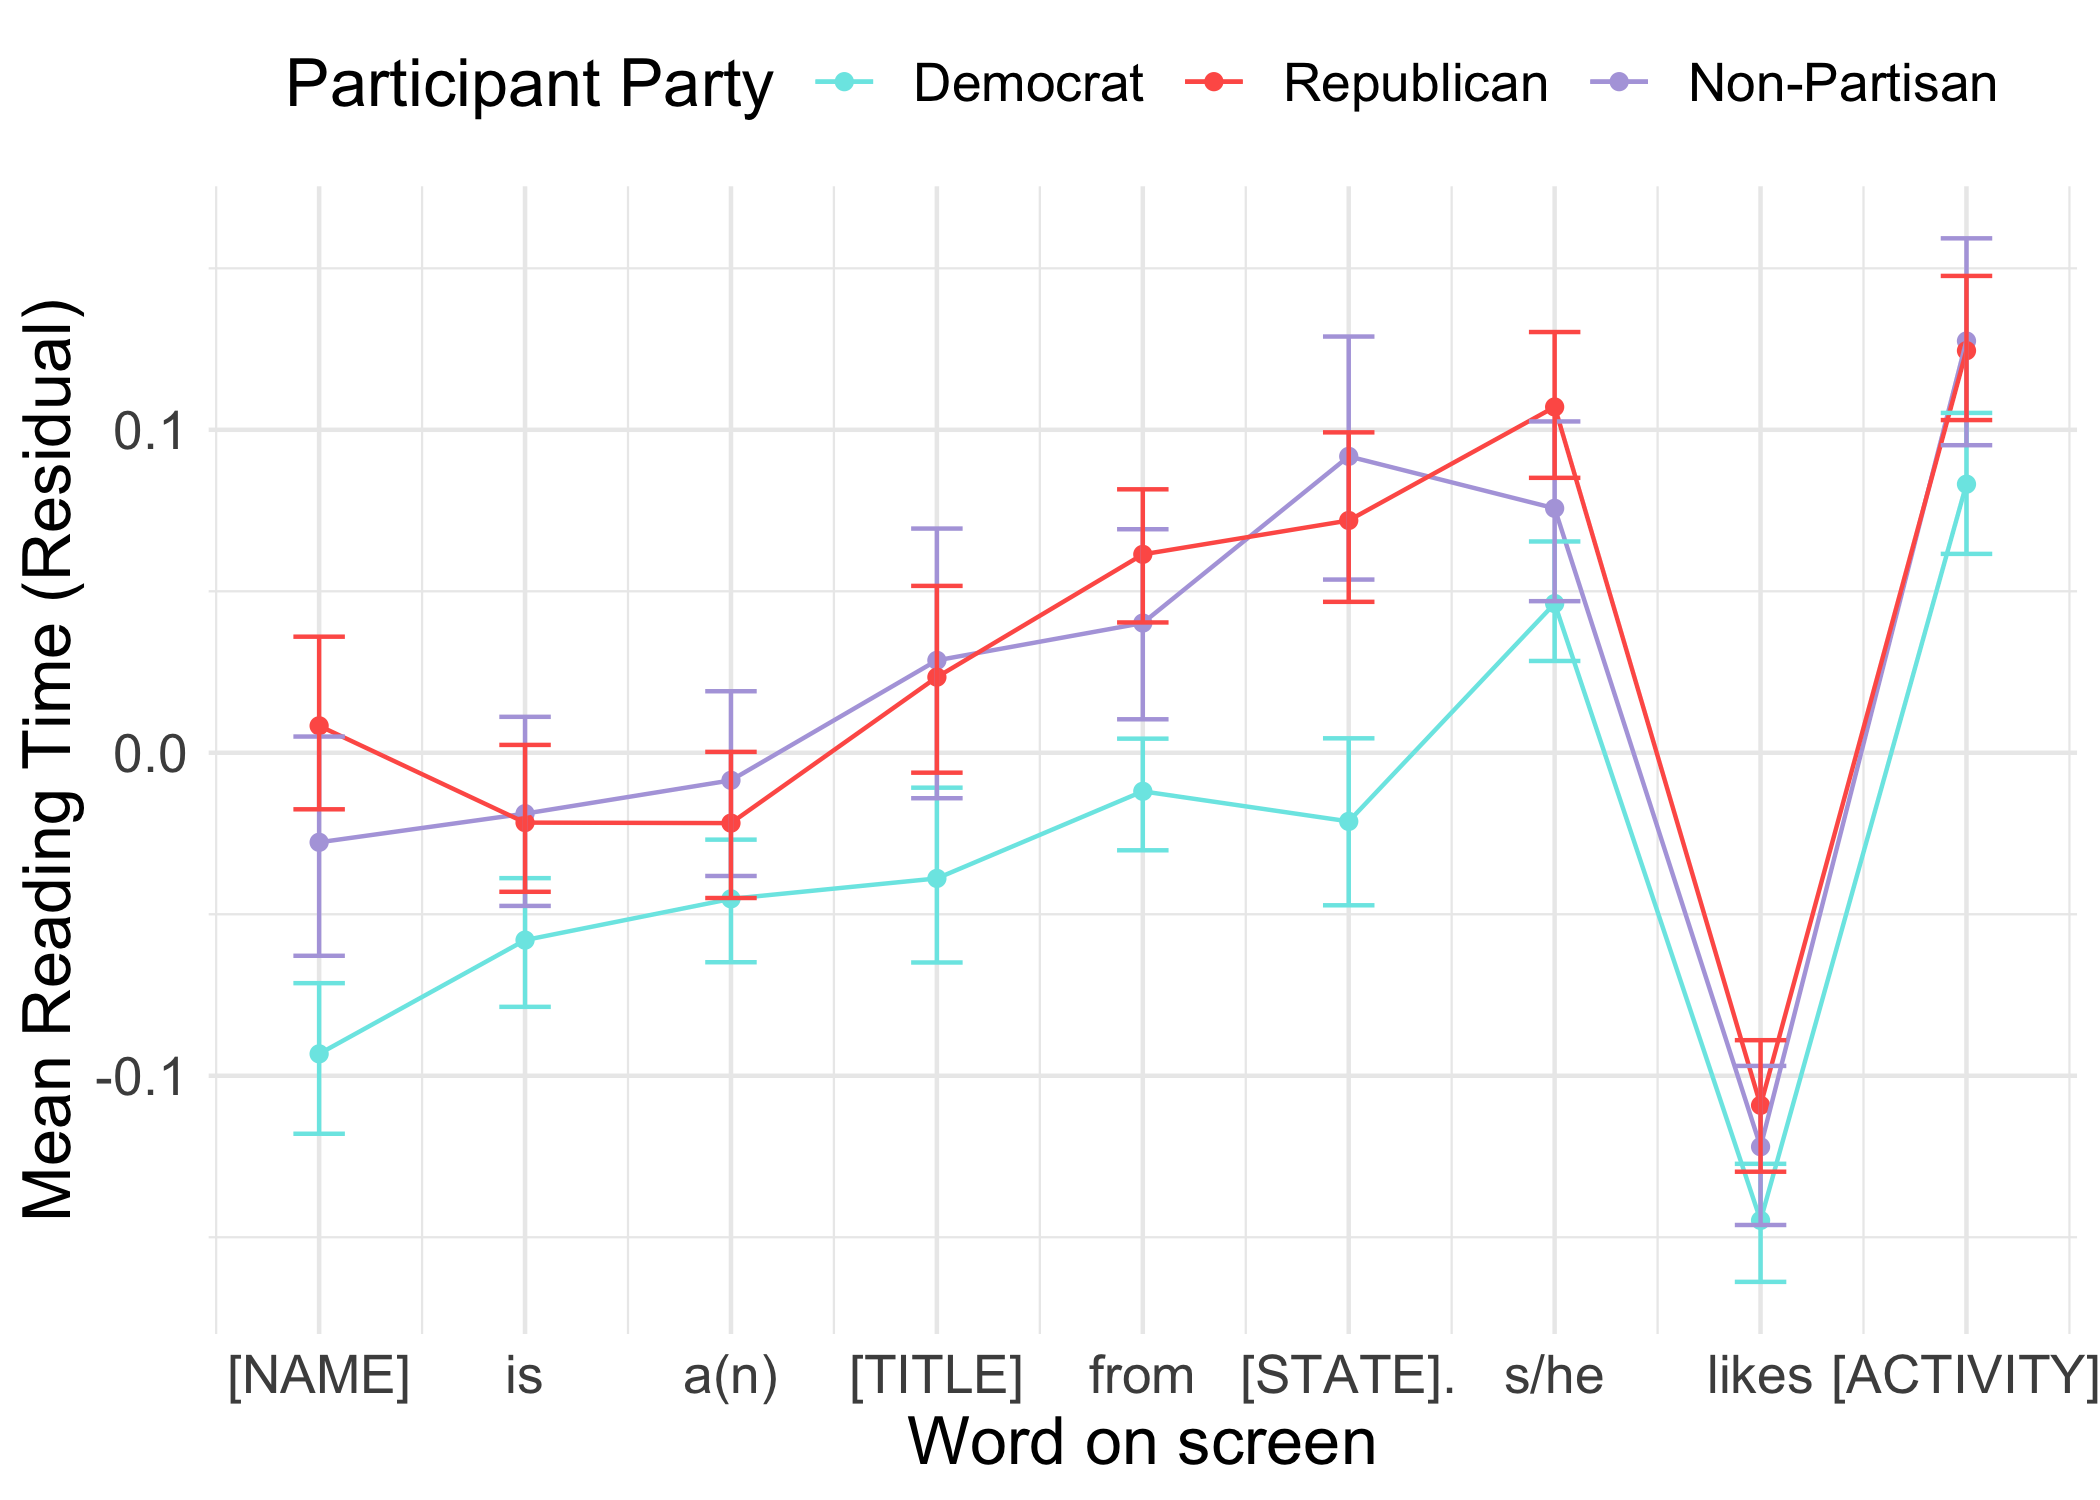
\includegraphics[scale=0.18]{sprt-neutral-all-regions-poli-party.png}
 	\caption{Residualised reading time at the different sentence locations in Experiment One. ``[TITLE]" indicates the location of the critical items.}
 \end{figure}

\newpage
   . 
\newpage
 
 	\begin{figure}[h]
 	\centering
 	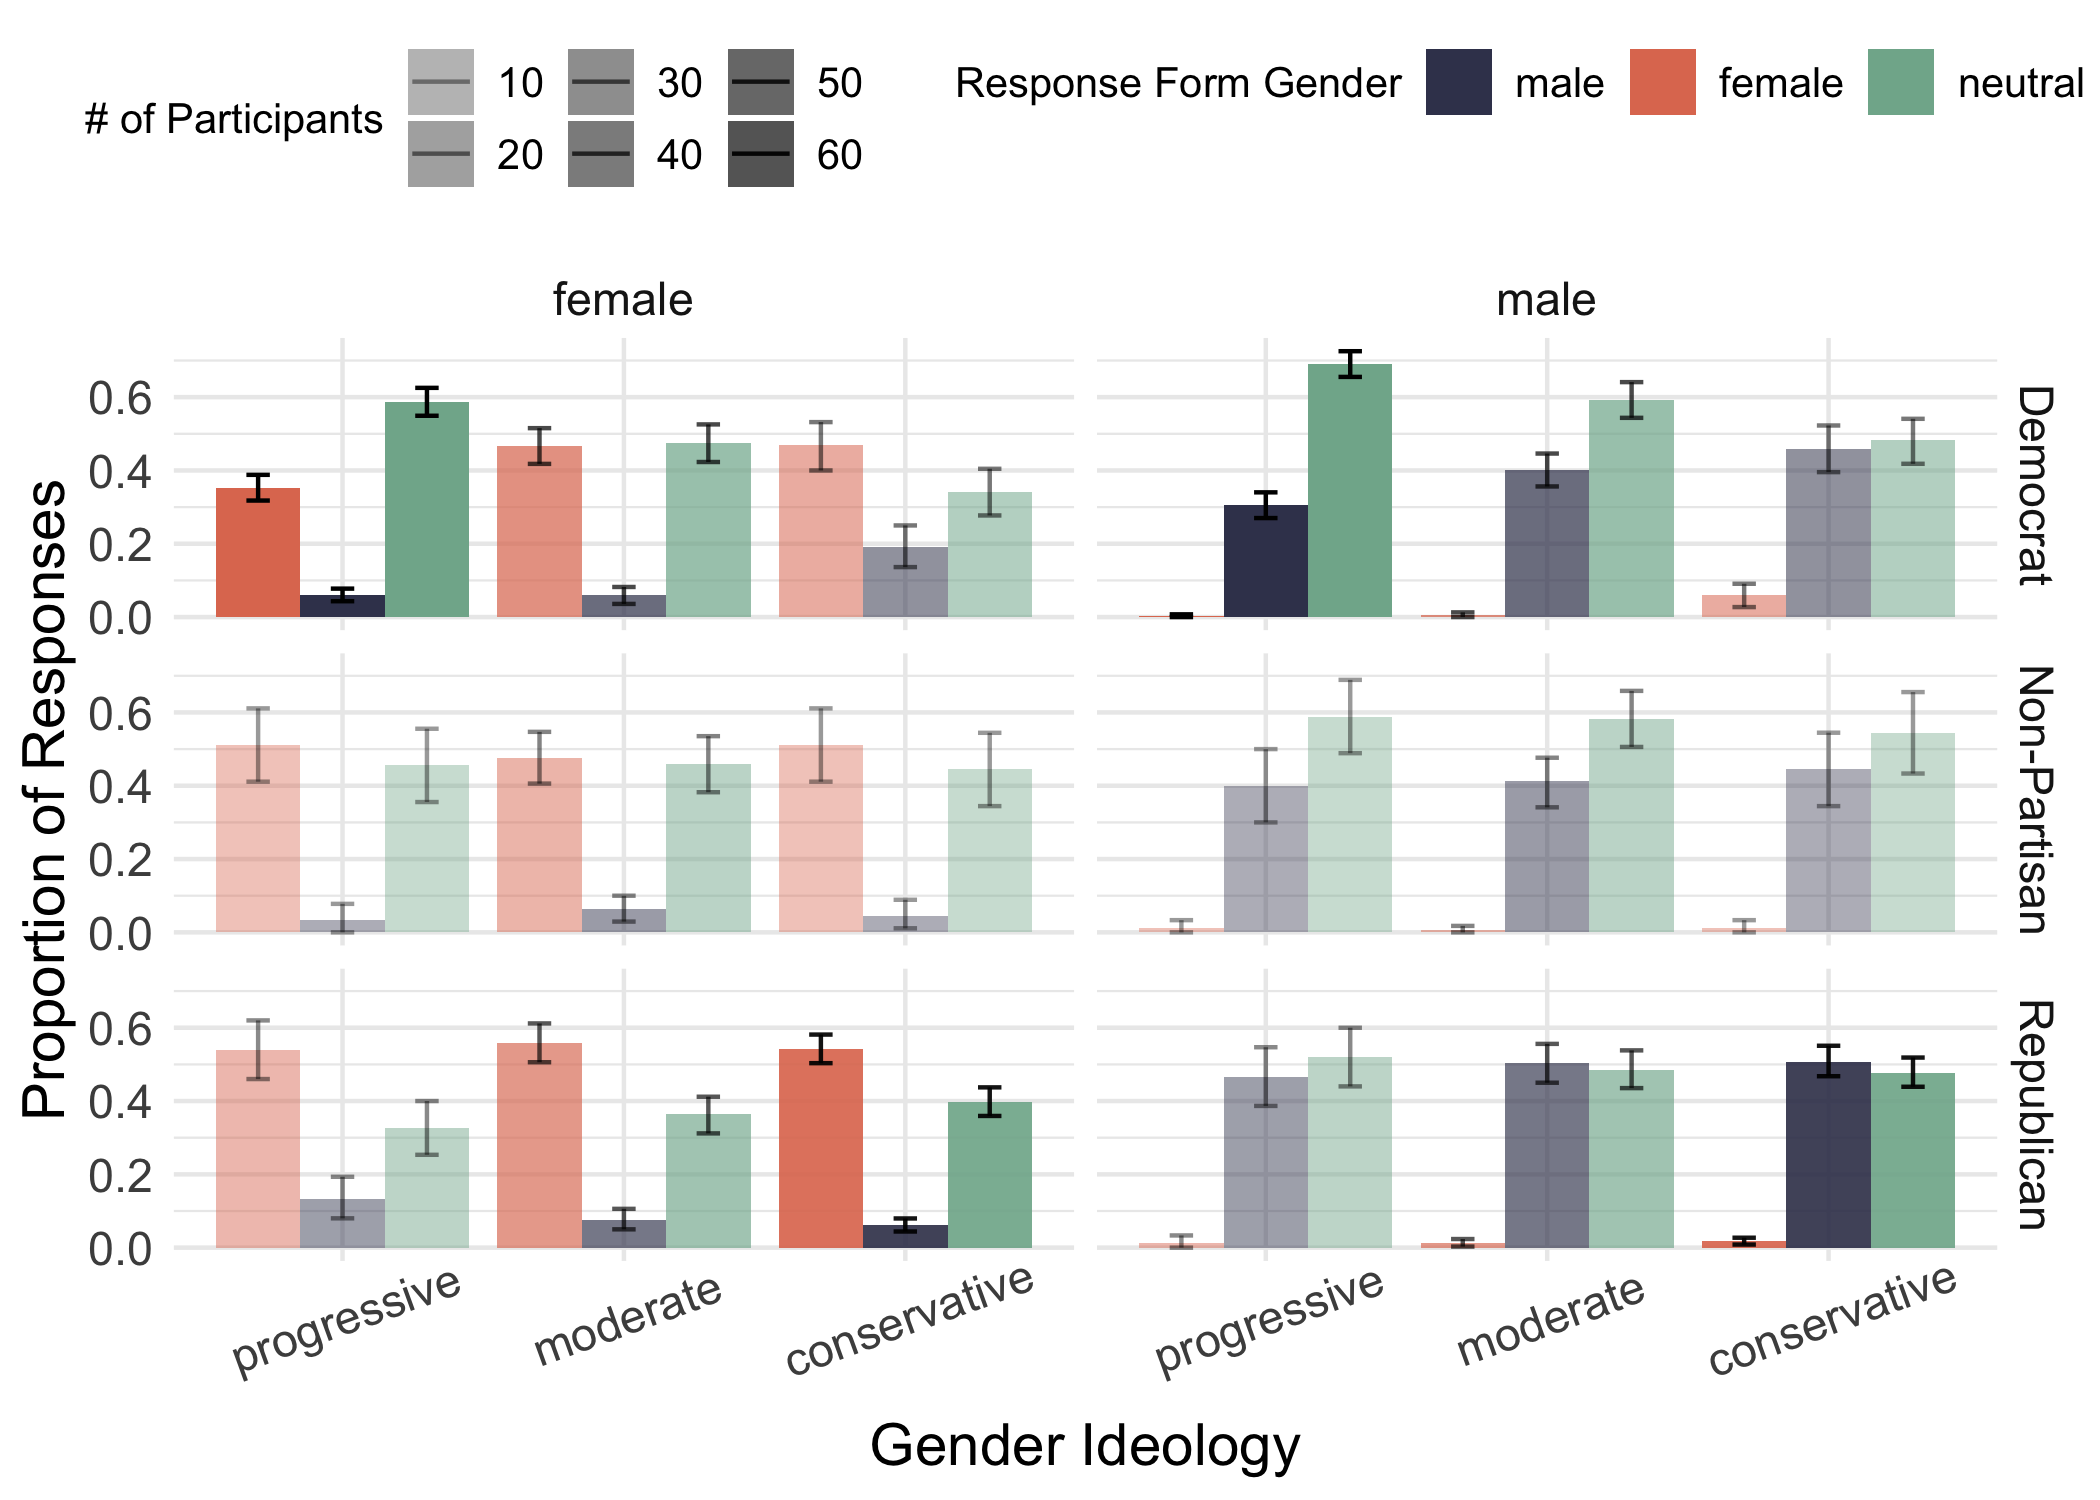
\includegraphics[scale=0.2]{prod-3x2x3.png}
 	\caption{Proportion of responses by gender produced in Experiment Two, according to gender of the name in the stimulus sentence (x-axis facet) and participant political alignment (y-axis facet)}
 \end{figure}

\newpage
. 
\newpage

\begin{figure}[h]
	\centering
	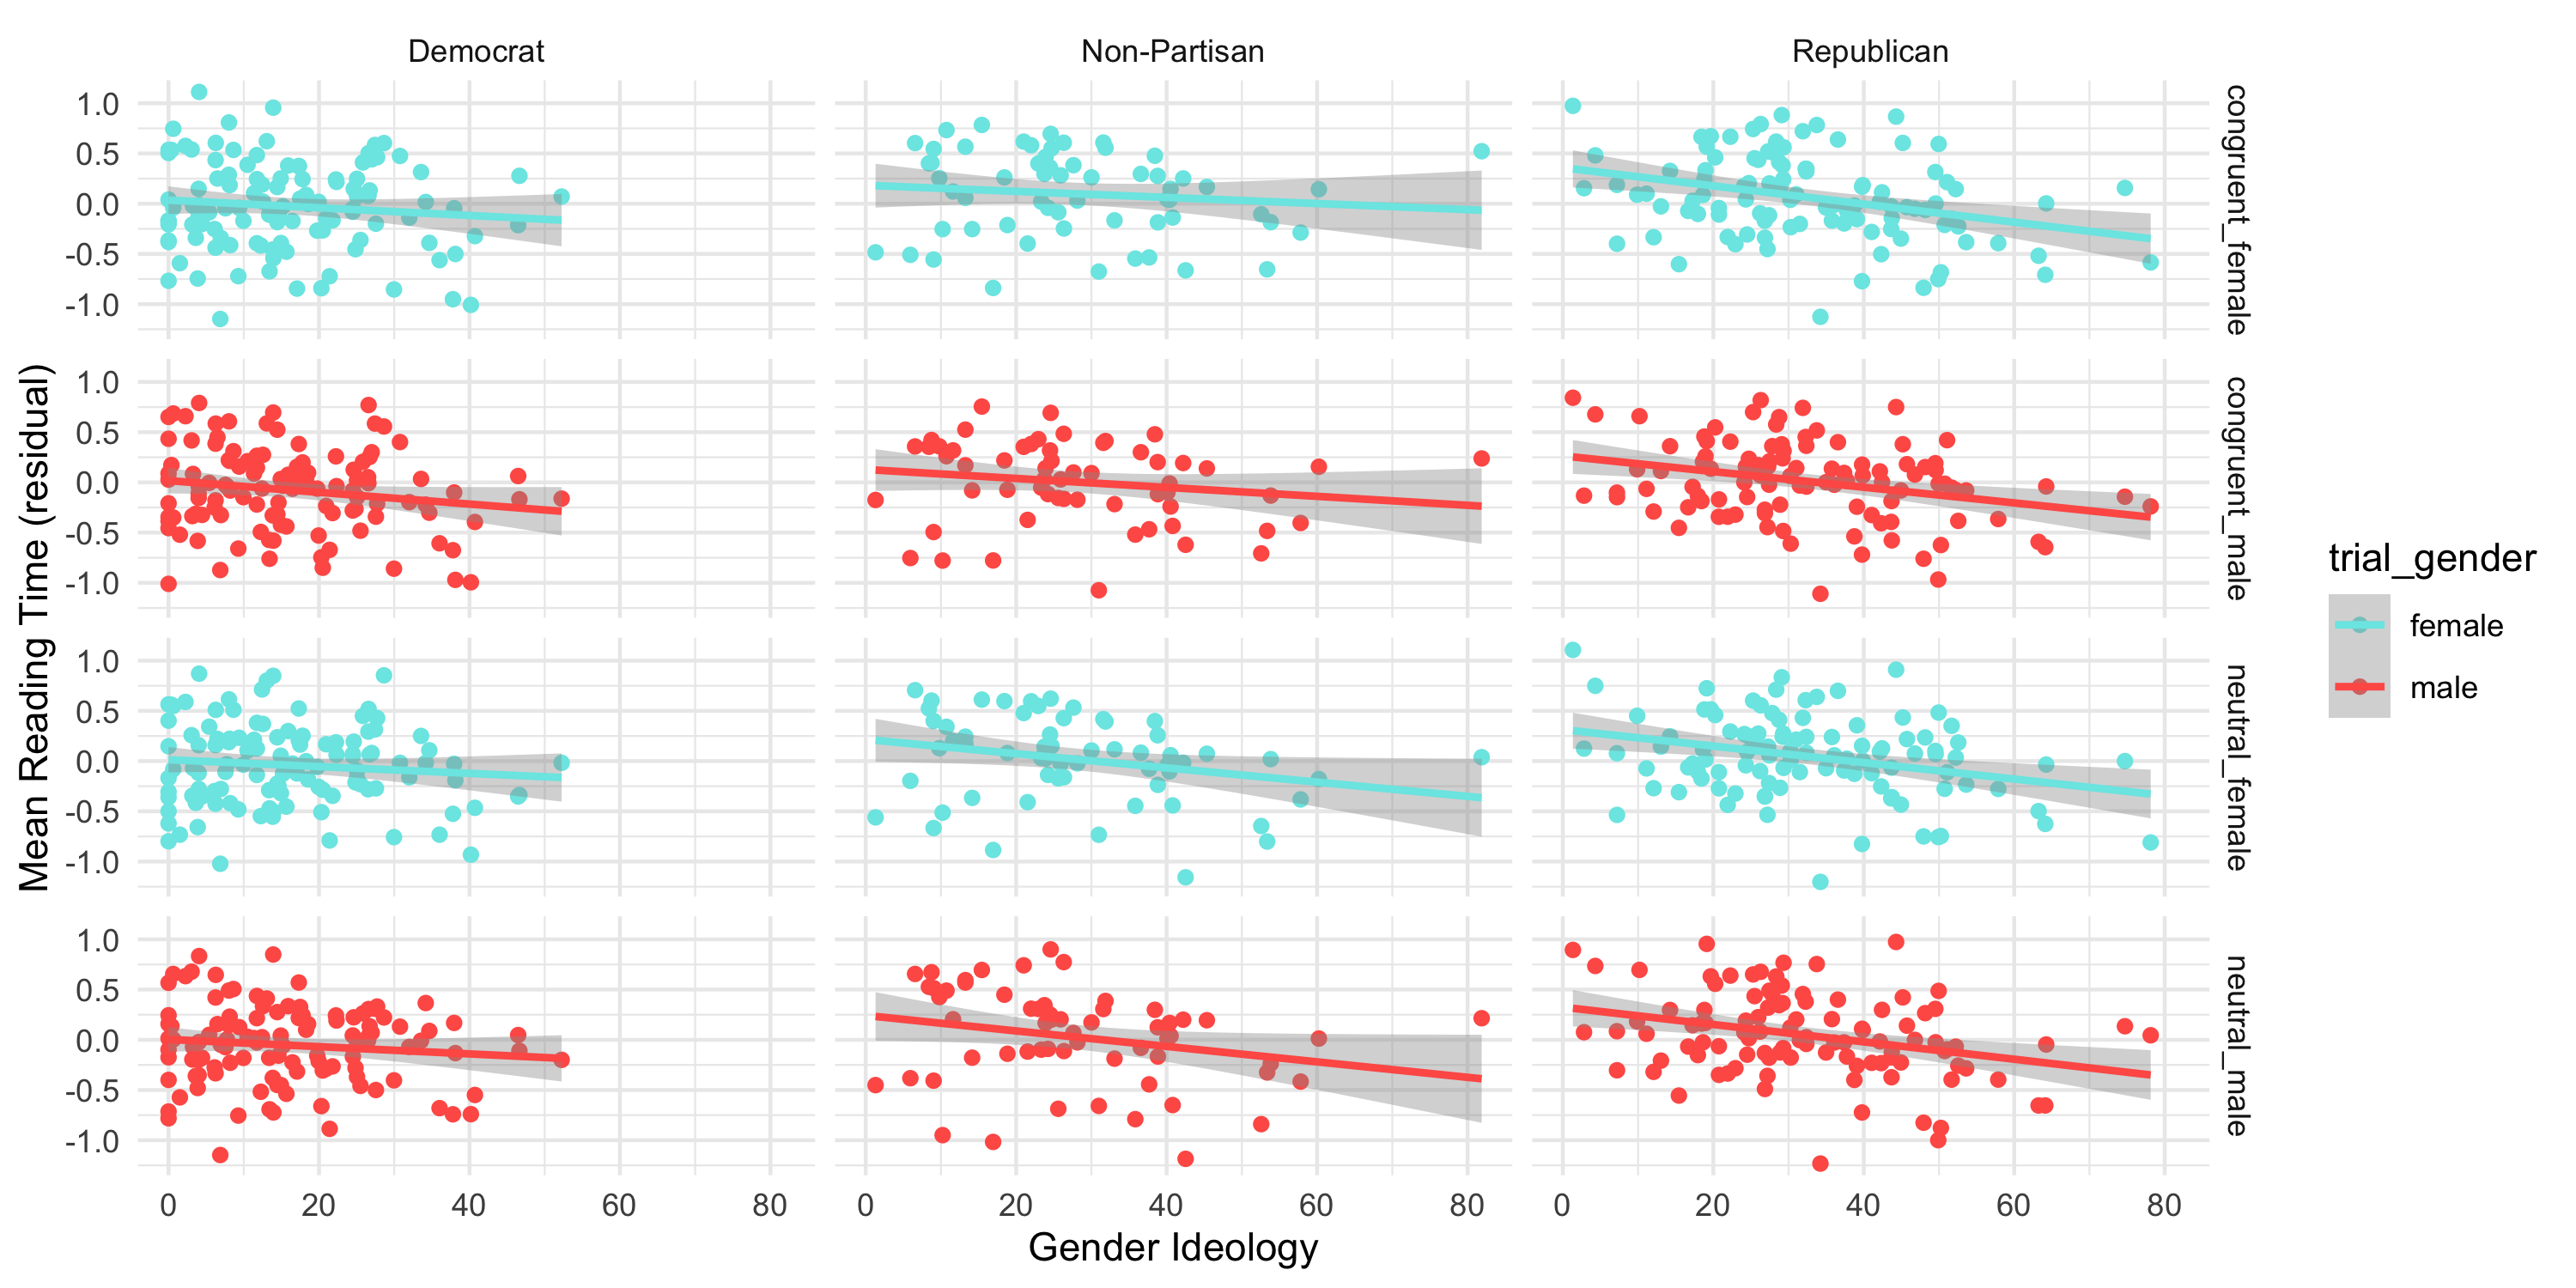
\includegraphics[scale=0.18]{sprt-neutral-3x3.png}
	\caption{null}
\end{figure}

 
 \begin{table*}
 	\centering
 	\caption{Model outputs for each fixed effect (rows) for each of the political macrocategories. Significant cells are shaded.}
 	\vskip 0.12in
 	\begin{tabular}{l r r l r r l r r l }
 		%		\begin{tabular}{l {p{2cm} r  p{2cm} r p{2cm} l p{2cm} r p{2cm} r p{2cm} l p{2cm} r p{2cm} r p{2cm} l }
 				\toprule
 				& \multicolumn{3}{c}{Democrats} & \multicolumn{3}{c}{Non-Partisans} & \multicolumn{3}{c}{Republicans} \\ \cmidrule(r){2-4} \cmidrule(r){5-7} \cmidrule(r){8-10}
 				& \multicolumn{1}{c}{$\beta$} & \multicolumn{1}{c}{SE} & \multicolumn{1}{c}{p} & \multicolumn{1}{c}{$\beta$} & \multicolumn{1}{c}{SE} & \multicolumn{1}{c}{p} & \multicolumn{1}{c}{$\beta$} & \multicolumn{1}{c}{SE} & \multicolumn{1}{c}{p}\\ 
 				\midrule
 				trial gender   & 1.247e-01 & 2.000e-02 & \cellcolor{lightgray} $<$0.001        & 1.299e-01 & 3.397e-02 & \cellcolor{lightgray} $<$0.001 & 1.706e-01  & 2.199e-02 &  \cellcolor{lightgray} $<$0.001\\
 				ideology & -5.643e-03  & 1.197e-03 & \cellcolor{lightgray} $<$0.001            & -1.073e-03 & 2.420e-03 & 0.66           & 8.718e-04  & 1.05 & 0.9 \\
 				log odds & 7.639e-06 & 1.204e-06  &  \cellcolor{lightgray} $<$0.001            & 5.403-06 & 2.220e-06 & \cellcolor{gray} 0.015     & 9.011e-06  & 1.310e-06 & \cellcolor{lightgray} $<$0.001\\
 				\bottomrule
 			\end{tabular}
 			%\caption{lmer(suspectconvictionJustified ~ generation * condition + (1|storyreproduction), data=dfmodel); high correlation of fixed effects}
 			\label{tab:exp2results}
 		\end{table*}
 
 \newpage


\end{document}